Space Shooter was developed with cross-platform availability in mind, precisely for both PC and Android devices. Because of the difference in input devices available to the two platforms, player input had to be implemented for each group individually. It was therefore necessary to design and outline the player actions prior to any concerning implementation, and test each control system separately. In this game, the main actions a player may take are as follows:
\begin{enumerate}
\item\label{th:radnil} Accelerate the ship.
\item\label{th:finsim} Decelerate the ship.
\item\label{th:leftnoe} Fire the weapon.
\item\label{th:leftnoe} Steer.
\item\label{th:leftnoe} Restart the game on defeat.
\end{enumerate}
Unity provides a set of tools in its script API that enables developers to identify various device details on run time, opening the possibility of automatic choice of device specific input methods on game start. This needs to be done only once, during the initialization phase of the game scene. C\# supports such behaviour through the use of delegates, assigning the proper function to handle input based on device data.\\
\begin{figure}
  \centering
  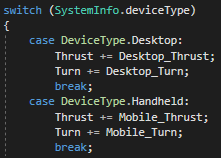
\includegraphics[width=0.6\linewidth]{images/inputdelegate}
  \caption{Dynamic input handling}
  \label{fig}
\end{figure}
As seen in Figure 4, Unity API provides an enumeration whose contents can be checked against the \textbf{SystemInfo.deviceType} value and the \textbf{Thrust} and \textbf{Turn} delegates are assigned to the proper implementation. This way the device specific code can be decoupled from the generic, common game components, enabling smooth and simple transition from one platform to the other. \\ 
In the case of a space shooter game, often times the Acceleration and Deceleration mechanics are considered unnecessary. In our sample game, those have been implemented for PC only, as it facilitated the presentation of various game data. On the Android platform, the player ship will always move with maximum velocity. \\ \\
After another glance at Figure 2.b, there is another UI element to be noticed, the two bars in top left, red and cyan. These are responsible for the survival mechanics. Red represents the ship's hull (health), while cyan represents the ship's force field (shield). Upon collision with an asteroid or an enemy projectile, first the shield is depleted, and then health points are deducted. The game ends when health points reach zero. While actual values are not displayed, they are proportionally reflected in the fill percentage of each bar. These bars, as UI elements, do not directly interact with other game objects, instead their attached scripts adjust the fill rate based upon player status data. \\
The asteroid field is composed of up to 2048 asteroids. They are initially created in a grid of 8 x 8 x 8, with minor random deviations to each axis. Each asteroid slowly moves on its set trajectory, which is also random. An asteroid can be destroyed by repeated projectile hits, or by collisions with other asteroids, drones or the player ship. Upon destruction, an asteroid breaks into two smaller asteroids, which also break into two yet smaller ones. These smallest asteroids do not break into smaller pieces, instead simply exploding upon destruction. \\
The space drones are static, up to 15 of them are randomly placed in the asteroid field. They will continuously rotate to face the player ship, and fire as often as possible. The space drones do not possess any movement mechanics, and do not have a shield. 